% Appendix G

\chapter{Určenie povrchového potenciálu $\varphi_{s0}$ pri nulovom napätí hradla.} % Main appendix title

\label{app:AppendixG} % For referencing this appendix elsewhere, use \ref{AppendixA}

\lhead{Appendix G. \emph{Určenie povrchového potenciálu $\varphi_{s0}$ pri nulovom napätí hradla}} % This is for the header on each page - perhaps a shortened title

Vo vzťahu \ref{eq:F.4} vystupuje výraz $\varphi_{s0}$, ktorý
predstavuje povrchový potenciál polovodiča štruktúry MOS v prípade, že
na štruktúru MOS nepôsobí žiadne vonkajšie napätie.  Tento potenciál
je spôsobený rozdielom výstupných prác kovu a polovodiča a nábojmi
nachadzájúcimi sa v izolante a na jeho rozhraní s polovodičom. Na
určenie tejto konštanty použijeme porovnanie nameranej a teoretickej
závislosti $\varphi_{s}$ od šírky OPN, ako je uvedené v
\cite{App.3}. Šírku OPN pre experimentálnu závislosť $\varphi_{s}(w)$
určíme zo vzťahu

\begin{equation}\label{eq:G.1}
w = \epsilon \Bigg[\frac{1}{C_{mos}^{HF}} - \frac{1}{C_{ox}}\Bigg]
\end{equation}

Pre určenie teoretickej závislosti $\varphi_{s}(w)$ použijeme
aproximáciu popísanu v \cite{App.5}

\begin{equation}\label{eq:G.2}
\beta \varphi_{s} = \frac{1}{2} \Big[\frac{w}{L_{DE}}\Big]^2 + \frac{1}{N_{B}L_{DE}^{2}} \int_{0}^{w}x[N(x)-N_{B}]dx + 1
\end{equation}

kde $L_{DE}$ je extrinzická Debayova dĺžka, $N_{B}$ koncentrácia
substrátu a $N(x)$ priebeh koncentrácie dotujúcich prímesí v
podpovrchovej oblasti polovodiča. Na obrázku \ref{fig:App.3} je
znázornený priebeh uvedených závislostí pre namerané dáta Q-C metódy z
obrázku \ref{fig:3.4}. Hodnotu $\varphi_{s0}$ potom určíme z rozdielu
experimentálnej a teoretickej závislosti $\varphi_{s}(w)$ v hĺbke w,
ktorá zodpovedá stavu ochudobnenia štruktúry MOS. Ako je uvedené v
\cite{App.3} aproximácia \ref{eq:G.2} ignoruje voľné nosiče náboja, z
čoho vyplýva jej obmedzenie platnosti len pre stav ochudobnenia.
Uvedeným spôsobom možno vypočítať aj integračnú konštantu pri výpočte
závislosti $\varphi_{s}(V_{g})$ pomocou Berglundovho integrálu.

\begin{figure}[h!]\centering
%\framebox[10cm]{\rule{0cm}{3cm}}
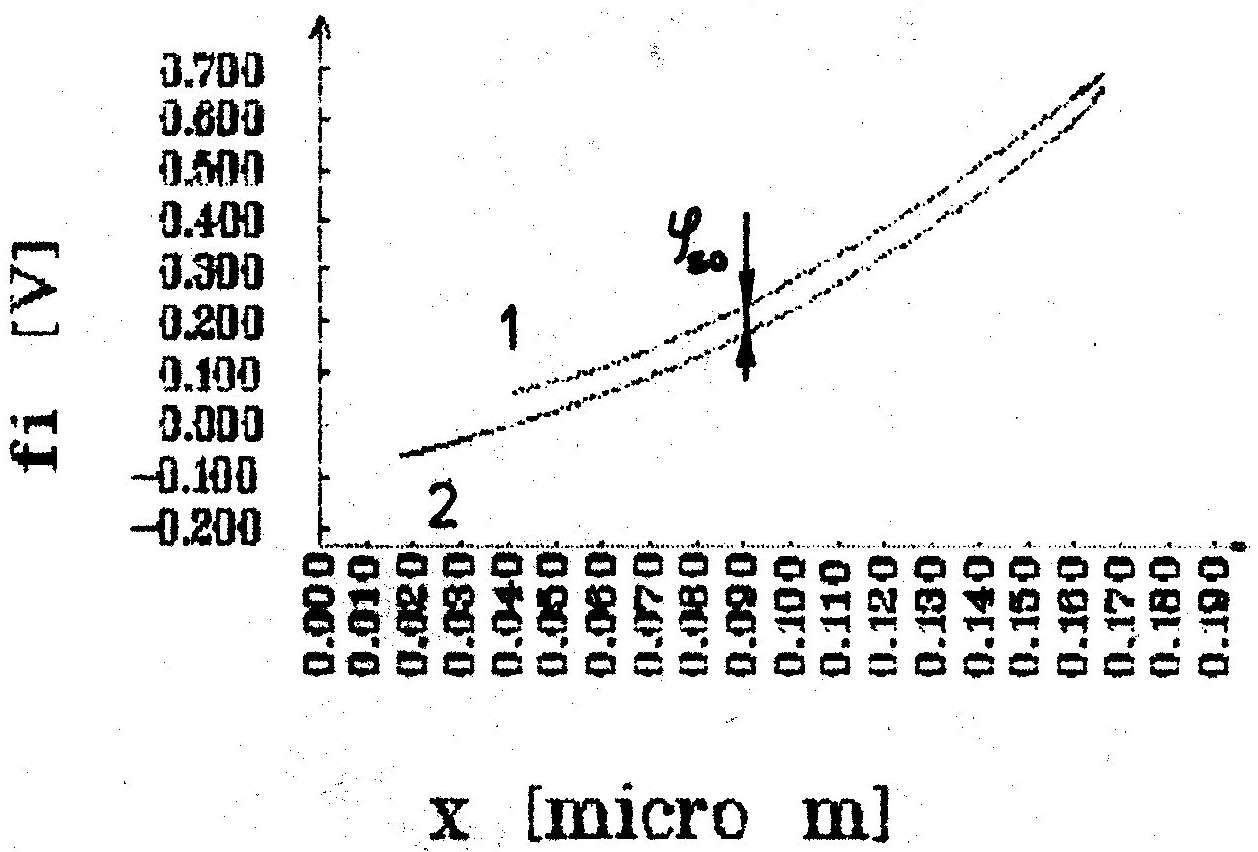
\includegraphics{Figures/fig-app-3.eps}
\captionsetup{justification=raggedright, singlelinecheck=false}
\caption[Priebeh povrchového potenciálu ako závislosti šírky OPN pre
  štruktúru MOS privedenú do stavu hlbokého ochudobnenia]{Priebeh
  povrchového potenciálu ako závislosti šírky OPN pre štruktúru MOS
  privedenú do stavu hlbokého ochudobnenia.  Krivka 1 predstavuje
  priebeh $\varphi(x)$ vypočítaný podľa vztahu \ref{eq:G.2} a krivka 2
  znázorňuje závislosť určenú z experimentálnych dát pomocou vzťahu
  \ref{eq:F.4}.}
\label{fig:App.3}
\end{figure}
% OBR10.BIT
